% AndroNet camera-ready paper. Generated into andronet.tex by build_paper.py, which fills every
% measured value from evaluation/results/. Edit this template, never the generated file.
\documentclass[runningheads]{llncs}
\usepackage[T1]{fontenc}
\usepackage{newtxtext}
\usepackage[varvw]{newtxmath}
\usepackage{graphicx}
\usepackage{booktabs}
\usepackage{pifont}
% The corresponding author's envelope, from ZapfDingbats, a Type~1 font; bbding's would embed as a bitmap
\newcommand{\Envelope}{\ding{41}}
\usepackage{url}
\urlstyle{same}
\begin{document}

\title{AndroNet: Privilege-Adaptive Packet Capture and On-Device Multi-Layer Threat Detection for Android}
\titlerunning{AndroNet: Privilege-Adaptive Capture and On-Device Detection}

% Springer cannot change authors after the files are delivered. One corresponding author is marked
% by \Envelope and must have an email address. ORCIDs, when available, go after each name as
% \orcidID{0000-0000-0000-0000}.
\author{Swastik\Envelope \and
Ritik \and
Kamal Akhter \and
Syed Misbah Uddin}
\authorrunning{Swastik et al.}
\institute{Department of Computer Science and Information Technology,\\
Central University of Jammu, Samba 181143, Jammu and Kashmir, India\\
\email{swastik362004@gmail.com, ritikrajput147@gmail.com,}\\
\email{kamalakhter694@gmail.com, bytesyed@gmail.com}}


\maketitle

\begin{abstract}
Network intrusion detectors must infer who is talking from addresses and ports. A phone's operating system already knows which app owns each connection, yet Android monitors mostly use that knowledge to label traffic. AndroNet puts it to work for detection. The open-source analyser captures traffic without root through a local VPN, or with root at the interface, and runs four detection layers on the handset: statistical detectors and stateful rules that count per app, payload signatures, and flow-level tests that need no decryption, including a per-app profile of TLS libraries. We evaluated it on physical phones in two frozen cycles. The first uncovered defects that unit tests had hidden and cut flagged benign packets from 33.9\% to 0.022\%. The second replays frozen versions over 45 third-party captures unopened until the freeze. Counting only alerts on an attack's own flows, recall rises from 7 to 11 of 24 in-scope captures, including 3 of 8 Android trojans, with 0.0019\% of phone packets flagged. Switching app identity off adds two false alarms in a session and stops alerts naming the app. Through the full pipeline the phone moves 160~Mbit/s down and 173 up, level with PCAPdroid, and keeps quiet connections that PCAPdroid drops, at the cost of more CPU and memory. In 41 hours of everyday use on two phones it raised 37 alerts and hit Android~15's six-hour daily cap on capture, now fixed. The VPN path stays blind to inbound scans, which the rooted path catches on an emulator.

\keywords{Mobile network security \and Intrusion detection \and Android VpnService \and Application identity \and On-device analysis.}
\end{abstract}

\section{Introduction}

Ask a network analyst to look at suspicious traffic and they will open Wireshark without a second thought. Ask the same of the phone in their pocket and the habit fails, because packet analysers expect interface access, raw sockets and spare CPU and memory, none of which Android gives an ordinary app.

Capture is no longer the hard part. The VpnService API~\cite{vpnservice} lets an unprivileged app route device traffic through a local tunnel~\cite{antmonitor,razaghpanah}, and PCAPdroid~\cite{pcapdroid}, the best-known open-source tool of this kind, offers that route alongside a root mode. The open question is what happens to the traffic next. PCAPdroid can flag hosts on third-party blocklists~\cite{pcapdroiddocs}, while payload signatures and multi-packet behaviour remain the territory of Snort~\cite{snort} and Zeek~\cite{bro}, which on a phone need a rooted chroot such as Kali NetHunter~\cite{nethunter}.

The phone has one thing those systems lack: it knows which app sent each packet. A network sensor only sees addresses, and inside a VPN tunnel every outgoing packet carries the same source address, so a detector counting per source ends up counting the whole phone. Counting per app keeps a browser's page load apart from a background app's burst of connections. It also lets us ask what no network sensor can: whether an app still uses the TLS library it has always used.

AndroNet is built around that advantage. Its root-free and rooted back-ends feed one pipeline of protocol dissection and four detection layers, with no server or tethered host. We evaluated it in two frozen cycles. In the first, a version that passed all of its unit tests flagged over 40\% of ordinary packets the first time it ran on a phone. In the second, the corrected and extended system faced third-party captures that no development decision had seen, Android remote-access trojans among them. Our contributions are:
\begin{enumerate}
\item \textbf{App-attributed detection:} rate windows, thresholds and beacon tracking kept per app, and a per-app profile of TLS libraries (Sect.~\ref{sec:detection}), with the value of app identity measured by switching it off (Sect.~\ref{sec:identity}).
\item \textbf{Detection for traffic it cannot read:} tests on how a flow opens, when it talks and what DNS says about it (Sect.~\ref{sec:layer4}).
\item \textbf{One analysis path over two capture back-ends, at relay speed,} with a bounded queue between relay and detection (Sect.~\ref{sec:architecture}).
\item \textbf{A measured evaluation on physical phones:} frozen versions on unseen captures, cost per core class, throughput and energy against PCAPdroid, and everyday use (Sect.~\ref{sec:evaluation}). Code, harness and results are public~\cite{repo}.
\end{enumerate}

\section{Background and Related Work}\label{sec:related}

\subsection{Capture and Detection}

Android apps cannot open raw sockets, so the usual workaround declares the app a VPN, reads outbound traffic from a TUN descriptor and relays it through sockets the app owns, as Lumen~\cite{razaghpanah} and AntMonitor~\cite{antmonitor} do. Inbound header fields are then synthesised, and only connections the device itself starts enter the tunnel~\cite{pcapdroiddocs}. PCAPdroid~\cite{pcapdroid}, the system closest to ours, relays with the zdtun library~\cite{zdtun} that AndroNet also uses, classifies flows, can decrypt TLS through a mitmproxy add-on, and analyses rooted captures through the same interface.

Snort~\cite{snort} set the pattern for signature matching, and Bro, now Zeek~\cite{bro}, for stateful analysis of network events. Attacks are rare, so the false alarm rate largely decides whether a detector is usable~\cite{baserate}, which is why we report false alarms on real phone traffic and kept third-party captures out of development.

\subsection{Detection on the Phone}

AndroIDS~\cite{androids} brought Snort-style signatures to Android in 2013 through an iptables queue, which needs root, and published no measurements. Chen et al.~\cite{chen2021} built an intrusion prevention system on VpnService and tcpdump, but we could find neither an open implementation nor cost and energy figures. Commercial mobile security products are closed, and we found no accuracy or cost data for them. Small open prototypes such as Syrrak~\cite{syrrak} apply rate and flow rules to the headers of VpnService traffic, apparently without evaluation. HydraDragonAV Mobile~\cite{hydradragon} comes closest to our use of app identity. It attributes connections to apps and scores them from blocklists, permissions and DNS behaviour, though its documentation mentions no payload, rate or TLS fingerprint detection and gives no accuracy figures. A 2026 study trains classifiers for an app derived from PCAPdroid, tests them on a public dataset, and leaves on-device latency and energy to future work~\cite{khalemskii}.

\subsection{App Identity and Encrypted Traffic}

Razaghpanah et al.~\cite{razaghpanah} used Lumen to fingerprint the TLS handshakes of 7,258 Android apps and found that about 84\% rely on the platform's default TLS API, in a study aimed at measurement alone. Matou\v{s}ek et al.~\cite{matousek} found JA3~\cite{ja3} hashes insufficient to identify a mobile app from the network, though fingerprints stayed fairly stable over time. Both results shaped our design. Identifying the app is the hard part for a network observer, and on the handset it comes for free, which leaves the easier and more useful question of whether a known app has changed. For traffic with no recognisable handshake, Wu et al.~\cite{wu2023} described how the Great Firewall of China spots fully encrypted flows from their first packet, and we turn their exemptions into a detector.

\section{Threat Model and Design Goals}\label{sec:threat}

AndroNet runs on the device whose traffic it watches, operated by its owner or an authorised assessor. It raises alerts and blocks nothing. The adversaries we consider leave traces in the device's own traffic: a malicious app or implant beaconing to command-and-control servers or exfiltrating data, an attacker on the same network segment who scans, floods or tampers with ARP, and hosts showing recognisable attack tooling. An adversary with kernel-level control of the device can defeat any analyser running on it, so that case is out of scope.

Four goals shaped the design: \textbf{G1}, useful analysis on unmodified consumer devices, with root adding visibility; \textbf{G2}, nothing above the capture tier branching on capture mode, only on whether a record names an app; \textbf{G3}, detection on the handset, within a per-packet budget and never holding up forwarding; \textbf{G4}, output that desktop tools can read.

\section{System Architecture}\label{sec:architecture}

AndroNet is split into three tiers: a Flutter interface, a Kotlin service layer and a C native layer (Fig.~\ref{fig:architecture}). On launch it checks for a working \texttt{su}. Rooted devices take the root path and all others the VPN path, though the user can override the choice. Both paths build the same record, defined in a single source file, and pass it to one pipeline.

\begin{figure}[t]
\centering
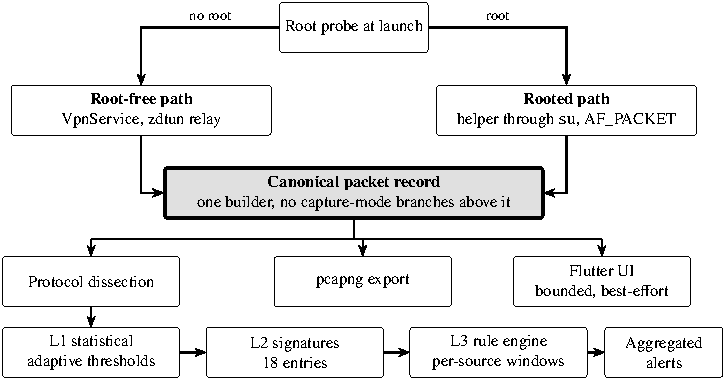
\includegraphics[width=0.9\textwidth]{fig_architecture.pdf}
\Description{Block diagram. A root probe selects between a VPN capture path on the left, which relays traffic through a bounded queue and knows the owning app, and a root capture path on the right, which sees inbound and link-layer traffic. Both feed a canonical packet record in the centre. Below it, protocol dissection feeds four detection layers, statistical, signature, rule engine and flow and app detectors, which feed alerts. Export and a bounded user interface stream also read from the record.}
\caption{AndroNet's architecture. The canonical packet record is the abstraction boundary: nothing below it knows which capture path produced a packet, only whether the record names an app.}\label{fig:architecture}
\end{figure}

\subsection{The Packet Record and the Capture Paths}

Every captured packet becomes one record: addresses and ports, protocols, size and capture timestamp, TCP flags, capture mode and direction, the owning app when the platform can resolve it, and, for ARP, the sender's address and MAC. On Android~10 and later the VPN path asks \texttt{ConnectivityManager} for the UID behind each connection and caches the app's label. The capture mode travels with the record for provenance only. No analysis component reads it, and a unit test checks that both modes raise identical alerts for identical bytes.

\textbf{Root-free path.} AndroNet declares a VpnService, obtains a TUN descriptor and relays traffic through zdtun~\cite{zdtun}, needing only the VPN permission the user grants. zdtun is not thread-safe, so a single loop owns it, draining the TUN descriptor and servicing its sockets. \textbf{Rooted path.} Even on a rooted device an app process cannot open a packet socket, so AndroNet launches a small helper through \texttt{su}. The helper opens one AF\_PACKET socket, drops to the app's user ID (the open socket survives the switch) and streams frames over standard output. It quits as soon as the app stops reading, so a crashed app leaves no capture process behind. Either way, AndroNet can export what it analyses as pcapng that Wireshark opens directly (checked on a 3{,}864-packet export from the Pixel~8).

\subsection{Keeping Detection off the Relay}\label{sec:relay}

Forwarding must never wait for detection. The relay drops each packet into a bounded queue (8192 packets or 32~MiB) and moves on, and a second thread analyses it using the capture timestamp, so rate windows follow traffic time and ignore queueing delay. A packet that finds the queue full is forwarded without analysis. Those skips are counted and raise an alert, since otherwise an attacker could blind the analyser simply by flooding it. Payload inspection stops after 64~KiB per direction of a cleartext flow and 8~KiB of an encrypted one, the trade Suricata makes with stream depth and encryption handling~\cite{suricata}, while headers, rates and sizes keep feeding detection and export still gets whole packets. The tunnel MTU is 10,000 bytes, as in PCAPdroid, because zdtun forwards one segment per pass of its loop, and the interface stream pauses while the app is in the background. Left alone, zdtun resets a TCP connection after 60~s of silence and breaks the connections phone apps keep open for push messages, so version 1.5.1 builds it with the idle limits RFC~4787 and RFC~5382 ask of a NAT, and room for 512 sockets.

\subsection{Dissection and DNS Visibility}

The dissection stage reads HTTP on any port (request line, percent-decoded URL, status, headers), DNS (question, record types, answers, response code) and TLS on any port (version, Server Name Indication, and JA3~\cite{ja3} and JA4~\cite{ja4} fingerprints). Hellos split across segments are reassembled up to 16~KiB, with no key material involved. Once GREASE values that Wireshark~4.6.5 keeps in signature algorithms are removed, both fingerprints match Wireshark's on 4{,}426 of 4{,}426 hellos from phone and enterprise captures.

Android moves its resolver to DNS over TLS or HTTPS whenever the server supports it, and names then vanish; on the Pixel~8 not one plain DNS packet crossed the tunnel. AndroNet refuses those encrypted connections inside the tunnel, so the resolver falls back to plain DNS that detection can read. The price is that DNS leaves the phone unencrypted while capture runs. A user who chose a strict Private DNS server keeps it, since Android has no fallback in that mode, and the DNS detectors then see nothing.

\section{Four-Layer Detection Engine}\label{sec:detection}

Every enriched packet passes through four independent layers. Detectors count per \emph{principal}: the app where the record names one, otherwise the source address, as on the rooted path. All state is bounded. Findings are aggregated, so repeats of one finding about one principal within 10~s yield a single alert, as with event filtering in Snort, and each alert names the app where known.

\subsection{Layer 1: Statistical Detectors}

Table~\ref{tab:l1} lists the detectors. During a 60~s learning period, with alerts muted, each counter's per-second peak is recorded. The threshold is then set to $2.5$ times the 90th percentile of those peaks, clamped between a floor and a ceiling, where the ceiling is the larger of the default and four times the learned baseline. From then on an exponential moving average ($\alpha=0.05$) tracks the baseline, but a sample that reached the threshold never trains it, so an attack cannot raise the bar it is measured against. A browser may open three times as many connections as other apps, because a page load legitimately fans out, an allowance only app identity makes possible. Distinct sources are counted with a 256-register HyperLogLog sketch~\cite{hyperloglog} per target, so a spoofed flood costs fixed memory however many addresses it forges.

\begin{table}[t]
\centering
\caption{Layer~1 detectors. Floors and defaults come from measured benign traffic.}\label{tab:l1}
\small
\begin{tabular}{@{}lll@{}}
\toprule
Detector & Trigger & Severity \\
\midrule
Port scan & destination ports from one principal in 10~s (floor 8, default 20) & High \\
SYN flood & SYN packets to one target per second (floor 50, default 100) & Critical \\
Distributed flood & 300 packets per second at a target, half from distinct sources & Critical \\
Connection flood & new connections per principal per second (floor, default 100) & High \\
DNS tunnelling & 10 query names over 50 characters under one zone in 60~s & Medium \\
ARP spoofing & binding changes, or one MAC claims two addresses (rooted path) & Critical \\
Malformed TCP & SYN set together with FIN or RST & Medium \\
Covert channel & high entropy in ICMP echo or outgoing HTTP or DNS, for 5 packets & High+ \\
\bottomrule
\end{tabular}
\end{table}

\subsection{Layers 2 and 3: Signatures and Rules}

The second layer matches 18 signatures in eight categories, built from patterns on payload content, named HTTP fields, ports, addresses and DNS names, combined with AND and OR. They include Meterpreter method names, Cobalt Strike's default User-Agent, scanner and login-tool fingerprints, and the WannaCry kill-switch domains. Two entries, the Tor exit and known-C2 lists, ship with sample indicators only, so real use needs a threat feed. A 64-byte tail kept per flow lets a pattern split across two consecutive segments still match.

The third layer evaluates 10 rules built from 26 predicates and the combinators And, Or and Not. They cover horizontal scans (over 100 destinations in 10~s, 300 for browsers), SQL injection, executable downloads, DNS tunnelling, brute force, cryptomining, bulk uploads (over 1~MiB per 10~s to one destination), shellcode, scanner User-Agents and ICMP tunnelling. Evaluation takes two passes. The first ignores rate predicates, and a packet that fails it is not the kind the rule counts, so it never enters the window. A packet that passes joins a window kept per rule and per principal, and the second pass evaluates rates over that window alone, so ``more than 10 per second'' means ten suspicious packets from this app. Each rule keeps at most 1000 entries for each of 64 principals.

\subsection{Layer 4: Flow and App Detectors}\label{sec:layer4}

Most phone traffic is encrypted, which leaves the layers above little to read. The fourth layer works from what any flow reveals anyway: which library opened it, what its first bytes look like, when it talks, and what DNS says about it (Table~\ref{tab:l4}).

\begin{table}[t]
\centering
\caption{Layer~4 detectors. All need no decryption, and APP-001 needs app identity. FLOW-001 to FLOW-003 report at most once an hour per principal and target.}\label{tab:l4}
\small
\begin{tabular}{@{}lp{0.66\textwidth}@{}}
\toprule
Detector & Trigger \\
\midrule
APP-001 new TLS library & a settled app presents a cipher list new to it \\
FLOW-001 opaque flow & first payload looks uniformly random, on a port with no expected encryption \\
FLOW-002 protocol mismatch & first payload on port 22, 53 or 80 does not speak that port's protocol \\
FLOW-003 beacon & gaps between bursts are regular, to a destination with no DNS or TLS name seen \\
FLOW-004 TXT channel & 3 TXT answers of 100 bytes or more under one zone in 60~s \\
FLOW-005 failed lookups & 20 distinct names fail to resolve for one principal in 60~s \\
\bottomrule
\end{tabular}
\end{table}

\textbf{TLS library profile.} Full JA4 values turned out too volatile to profile. In one phone session, 27 distinct values came from 4 cipher lists, because ALPN, the server name and resumption change the rest of the fingerprint from one connection to the next. AndroNet therefore profiles each app by the part of JA4 that hashes its cipher list. An app counts as settled after 20 consecutive hellos with no new list, and a new list from a settled app raises one alert and restarts settling. Profiles hold 16 lists for each of 256 apps and survive restarts. An implant that brings its own TLS stack into an app shows up here, and so does a plugin or a major library update, the false alarm this test accepts.

\textbf{Opaque first payloads.} We test a flow's first payload against the exemptions Wu et al.~\cite{wu2023} documented: bits set per byte outside 3.4 to 4.6, six printable bytes at the start, over half the bytes printable, a printable run over 20 bytes, or a recognisable TLS or HTTP start. A payload that earns none of these raises an alert unless its port is known to carry encryption. Port 5222 is excused too, after a live run showed WhatsApp's own encrypted protocol there.

\textbf{Mismatch and beacons.} Traffic on ports 22, 53 and 80 should open with an SSH banner, a DNS message or an HTTP method. For beacons we keep the last 16 gaps between activity bursts for each principal and destination. A flow looks like a timer when at least 12 gaps exist, their median lies between 10~s and 10 minutes, and three quarters sit within 10\% of the median. It raises an alert only if no DNS or TLS name has been seen for the destination, so push services, which have one, stay quiet. Using the median keeps a single long pause from hiding a timer.

\section{Evaluation}\label{sec:evaluation}

We ask six questions. How accurate is detection on traffic no development decision saw? What does app identity add? Do the two capture paths behave alike? What does analysis cost on real hardware? How does the whole system compare with PCAPdroid? And how does it behave in everyday use?

\subsection{Setup and Data}\label{sec:setup}

\textbf{Hardware.} Our main phone is a Pixel~8 (Tensor~G3, 8~GB RAM, Android~17, unrooted user build) on 802.11ax Wi-Fi, sharing an access point with the lab laptop. A second unrooted phone, a mid-range Samsung Galaxy M53 (MediaTek MT6877, 6~GB RAM, Android~16), ran the live scenarios, a browsing and app session, and shorter speed tests. Stock user builds cannot exercise the rooted path, so we ran it on an Android~16 x86-64 emulator image with root.

\textbf{Harness.} Replay experiments run the production Kotlin classes under ART on the phone, through \texttt{app\_process}, with the clock following trace time. Versions 1.5.0 and 1.5.1 each gave identical verdicts on the phone and a desktop JVM for all 47 traces of the second cycle (1{,}514{,}251 packets), even with different regular expression engines. Live experiments use a release build that differs from a normal one only in accepting scripted commands. Unless stated otherwise, measurements on the phone use version 1.5.1.

\textbf{Data.} Table~\ref{tab:data} summarises the two cycles. In the first, we fixed a split, froze version 1.4.0 with file hashes recorded~\cite{repo}, and only then replayed third-party captures labelled from their publishers' descriptions. New detectors can only be validated on new data, so that set then became development data for version 1.5.0. For the second cycle we chose captures by a fixed rule from names and descriptions, opening none: all eight remote-access trojans in Android Mischief~\cite{mischief}, three recorded on a physical phone and five on emulators; every StopDDoS flood capture~\cite{stopddos} up to 50~MB that the first cycle left unused; and every unused Bousseaden capture~\cite{bousseaden}, most showing Windows-domain techniques no detector targets, which we keep and score apart. We wrote the expected alerts first, recorded the captures' hashes, froze both versions~\cite{repo}, and replayed them on the same data.

\begin{table}[t]
\centering
\caption{Evaluation data. The source of every capture is listed in the repository~\cite{repo}.}\label{tab:data}
\begin{tabular}{@{}llrr@{}}
\toprule
Set & Traffic & Captures & Packets \\
\midrule
First cycle & third-party attack captures & 28 & 108{,}168 \\
(v1.5.0 development) & third-party benign captures, including bigFlows~\cite{tcpreplay} & 11 & 810{,}700 \\
 & Pixel~8 browsing, after the first freeze & 1 & 201{,}020 \\
Second cycle & Android remote-access trojans & 8 & 563{,}334 \\
(unopened) & floods, and a backdoor using domain generation & 16 & 624{,}791 \\
 & Windows-domain techniques, no detector targets & 21 & 6{,}890 \\
 & phone sessions after the freeze, browsing and apps & 2 & 319{,}236 \\
\bottomrule
\end{tabular}
\end{table}

\subsection{What Measurement Changed}\label{sec:defects}

Version 1.3.0 passed all 106 of its unit tests, yet its first measurement exposed, among others, a dissector and detectors that disagreed on field names, so URL signatures never fired; thresholds sampled per packet while counters still rose, so a 400~pps SYN flood raised no alert; rate rules counting all traffic from all hosts, with 95{,}673 false alerts on one phone session; quadratic regular expressions under ICU, at 7.7~ms per packet; and zdtun driven from two coroutines at once, which held the tunnel to 15~Mbit/s. The unit tests built their input records by hand, so stages could each pass while disagreeing. We now push real wire bytes through the whole pipeline in a contract test suite, part of the 208 tests that version 1.5.1 passes.

Real phones then corrected version 1.5.0 before its freeze. WhatsApp's first payload on port 5222 looks fully encrypted. Full JA4 values changed within one TLS library. ICMP errors quoting QUIC packets resembled a covert channel. Advertising hosts tripped a DNS rule that fired on single long names, and repeated lookups of the same hosts looked like domain generation. A page's burst of large post-quantum TLS hellos read as a bulk upload. Each case led to a narrower test, and no lab trace had shown any of them.

\subsection{Detection Accuracy}\label{sec:accuracy}

We report \emph{capture recall}, the share of in-scope attack captures that raise at least one expected alert, and the \emph{packet false positive rate}, the share of benign packets that raise any alert. For the second cycle we also report recall counting only alerts raised by the attack's own packets, and \emph{alert precision}, the share of all alerts that such packets raise. Table~\ref{tab:accuracy} gives both cycles.

\begin{table}[t]
\centering
\caption{Detection by version. The first cycle's set was development data for v1.5.0, so only the second cycle is an unseen test of it. v1.5.1 fixes one defect that the second cycle exposed, so neither set is an unseen test of that version.}\label{tab:accuracy}
\small
\begin{tabular}{@{}lrrrr@{}}
\toprule
Measure & v1.3.0 & v1.4.0 & v1.5.0 & v1.5.1 \\
\midrule
\multicolumn{5}{@{}l}{\emph{First cycle: 1.01~million benign packets}} \\
Capture recall (in scope) & 12/19 & 12/19 & 17/19 & 17/19 \\
Packet false positive rate & 33.9\% & 0.022\% & 0.021\% & 0.021\% \\
Alerts on benign traffic & 352{,}310 & 218 & 215 & 213 \\
Phone browsing: packets flagged & 48.8\% & 0.001\% & 0.000\% & 0.000\% \\
\midrule
\multicolumn{5}{@{}l}{\emph{Second cycle: captures unopened until the freeze}} \\
Capture recall, by the rule fixed in advance & & 7/24 & 14/24 & 11/24 \\
Recall on the attack's own flows & & 7/24 & 11/24 & 11/24 \\
\quad Android remote-access trojans & & 1/8 & 3/8 & 3/8 \\
\quad Floods & & 6/15 & 8/15 & 8/15 \\
\quad Domain-generating backdoor & & 0/1 & 0/1 & 0/1 \\
Alerts off the attack's flows & & 99 & 15 & 4 \\
Alerts on untargeted captures & & 0 & 0 & 0 \\
Phone sessions: alerts & & 33 & 6 & 5 \\
Phone sessions: packets flagged & & 0.0103\% & 0.0019\% & 0.0016\% \\
Alert precision & & 82.8\% & 96.8\% & 98.6\% \\
\bottomrule
\end{tabular}
\end{table}

\textbf{First cycle.} Version 1.3.0 ``detected'' SSH password guessing by alerting on every packet to port~22, and raised 352{,}310 alerts on benign traffic. Version 1.4.0 kept its recall honestly and cut those alerts to 218. Its misses pointed to the new detectors: a spoofed flood from 9{,}886 addresses, ARP poisoning with no binding change, a shell on TCP port~53 and commands in DNS TXT answers. Version 1.5.0 catches these, which is development evidence only. It still misses Nmap's version scan, which touches two ports, and a Meterpreter capture that begins mid-flow and so has no first payload to test.

\textbf{Second cycle.} By the rule fixed in advance, version 1.5.0 detects 14 of 24 captures and version 1.4.0 detects 7. That rule accepts an expected alert anywhere in a capture, and these captures come from phones in everyday use, so we then read the packet behind every alert~\cite{repo}. This check, written after the run, can only lower recall. Version 1.4.0 stays at 7, version 1.5.0 falls to 11, and we take these figures as the result. Eleven FLOW-003 alerts fell on connections to public web services, and in three captures they were the only hit. Each followed the end of a DNS entry's five-minute life: the connection outlived the entry that named its address, and the beacon test took the address for an unnamed one. Version 1.5.1 remembers a name once seen for that destination. On the same captures it raises none of those alerts and keeps all 11 detections, giving up only one beacon alert on a controller whose address had a name, in a capture FLOW-001 also catches. These captures produced the fix, so they cannot test it; the everyday-use results below can.

Among the trojans, FLOW-001 caught the first payload to the controller in two captures, and Saefko's IRC channel raises a signature that version 1.4.0 also has. The misses show the limits of what a first payload can tell. Ahmyth and a command-line AndroRAT open with printable text, AndroRAT with a structured and largely printable message, and DroidJack's controller with a six-byte header, so none of them looks random or matches a signature, and HawkShaw's capture shows only web and messaging services, with no controller outside port~443. Among the floods, five of version 1.4.0's six hits came from its ICMP tunnel rule firing on error messages that quote the flood. Version 1.5.0 reads ICMP data only from echo messages, after the same errors raised false alarms on QUIC traffic, which cost it three of those captures while the distributed-flood detector gained five. Neither version detects the domain-generating backdoor, whose capture holds 28 packets, and neither raises any alert on the 21 Windows-domain captures. Long attacks repeat their alerts, which flatters precision in every column.

\textbf{A yardstick.} Suricata~8.0.7~\cite{suricata} with the ET Open rules~\cite{etopen} (52{,}849 signatures, downloaded for this comparison), run on a desktop over the same captures and counting any alert on an attack's flows, reaches 14 of 24. Its rules name AhMyth and the domain-generating backdoor, and Saefko's IRC traffic raises them too. They stay silent on the controller flows of the other six trojans, two of which AndroNet's first-payload test catches, so signatures and flow tests miss different things, and together they reach 4 of 8 trojans. Of Suricata's 11 flood hits, seven come solely from IP reputation rules written years after these captures, and only one from a rule that names a denial of service, whereas AndroNet's come from rate alone. On the phone sessions it raises 56 informational alerts, none claiming an attack. Counting any alert, with rules newer than the attacks, favours Suricata, which also needs a separate host or a rooted handset.

We also ran 28 attack scenarios live on the Pixel~8 through the real tunnel, with the app's alert log as the only output. Of these, 28 raised their expected alerts, and all 44 alerts named an app: the attacking process in 43, and an unrelated app that APP-001 flagged in one. Frozen version 1.5.0 detected 27, raising no alert for failed lookups, which needs answers from the lab's DNS server. The laptop has two adapters on the network, so that server's answers could leave from an address the phone would reject. Once it answered from the address asked, the scenario fired in 10 of 10 runs, though we cannot show that this caused the miss. On the second phone, 28 did, and its browsing and app session raised no alerts over 179{,}730 packets. Because these scenarios resemble the development traces, this verifies the path end to end and makes no independent accuracy claim.

\subsection{What App Identity Adds}\label{sec:identity}

We ran frozen version 1.5.0 with app identity switched off, so that detectors count per source address as a network sensor must, over two consecutive 13-minute sessions on the same sites and apps. With identity on, the live session raised no alerts over 139{,}506 packets. Replaying those same packets without identity raised one, and the live session with identity off raised two over 98{,}403 packets, all of them the horizontal scan rule reading page loads as a scan. Of the 28 attack scenarios, version 1.5.1 detected 27 with identity off, losing only the TLS library change, which needs identity by definition. These counts are small and bound the claim: on this traffic identity spares a few false alarms and changes no other detection. Beyond that, an alert with identity names the app to remove, where without it every alert names the phone's address.

\subsection{Capture-Path Parity and Observability}\label{sec:parity}

Running the same 27 scenarios through the rooted path gave the same expected detections, direct evidence for goal G2; the one scenario left out needs app identity. Another 7 traces, injected as real frames on the interface and covering inbound SYN, FIN, NULL and Xmas scans, a SYN flood and ARP spoofing, each raised the expected alert. The helper exited within 5~s of the app being killed. These rooted runs used an emulator and a stand-in for \texttt{su}, so the rooted path has yet to run on a physical rooted handset.

Identical analysis does not mean identical visibility. Only the VPN path knows which app sent a packet, and only the rooted path sees inbound scans and floods, ARP and other link-level traffic, and inbound headers as sent. To confirm the blind spot, we scanned the phone with real nmap from the laptop during VPN-mode capture. Over three scans of 1000 ports each, the phone's kernel answered 3{,}000 probes with resets, so the packets did arrive, yet AndroNet raised no scan alerts, because unsolicited inbound packets never enter a VPN tunnel. Every VPN-based tool shares this blind spot, and it is the strongest reason to keep a rooted path.

\subsection{Per-Packet Cost}\label{sec:cost}

We cost each layer by ablation: a trace is replayed with the signature and rule lists emptied by reflection, so the production code needs no timers. Layer~4 runs inside the Layer~1 stage and is costed with it. On a Cortex-A715 mid core, replaying tcpreplay smallFlows, the rule layer dropped from 7.2~ms to 20~\textmu s per packet. Version 1.5.1 averages 105~\textmu s per packet (21 at the median, 336 at p95), enough for about 9{,}700 packets per second on one mid core, 13{,}700 on the big core and 2{,}600 on a little core. With the scheduler free to choose its core, the Samsung Galaxy M53 sustains about 8{,}500. After replaying the trace, detection state occupies 836~KiB of heap.

\subsection{Throughput, Energy and PCAPdroid}\label{sec:headtohead}

Table~\ref{tab:headtohead} compares no capture, PCAPdroid~2.0.2 and AndroNet on the same phone and network, with the conditions shuffled in each of five rounds. Figures are medians of 50~MB transfers, two per direction per round. For energy, a script on the phone logged battery current and voltage once a second over 150~s, with the cable out, the screen on at minimum brightness and three repetitions in rotating order. The current comes from the fuel gauge, so these figures are coarser than an external power monitor would give. We measured PCAPdroid's free build without writing a capture file, and did not test its paid blocklist feature.

\begin{table}[t]
\centering
\caption{Head-to-head on the Pixel~8. Throughput and connect time are TCP between phone and laptop. AndroNet~1.4.0, measured in an earlier session, ran its full app with a 1500-byte tunnel. Version 1.5.1 is shown forwarding alone, and as the full app with its interface in front or in the background. Power is whole-device, under a 10~Mbit/s download and at idle.}\label{tab:headtohead}
\small
\begin{tabular}{@{}lrrrrrr@{}}
\toprule
Measure & None & PCAPdroid & v1.4.0 & \multicolumn{3}{c}{v1.5.1} \\
\cmidrule(l){5-7}
 & & & full & forward & in front & in back \\
\midrule
Download (Mbit/s) & 181 & 183 & 39 & 163 & 177 & 160 \\
Upload (Mbit/s) & 158 & 153 & 47 & 180 & 163 & 173 \\
TCP connect (ms) & 24.6 & 38.1 & 30.0 & 28.6 & 34.9 & 34.3 \\
App CPU (\% of a core) & -- & 19 & 128 & 31 & 71 & 66 \\
Peak memory (MiB) & -- & 151 & 414 & 258 & 316 & 311 \\
\midrule
Power, 10~Mbit/s (W) & 1.27 & 1.34 & 1.59 & & & 1.26 \\
Power, idle (W) & 0.94 & 0.99 & 0.96 & & & 1.09 \\
Battery, 10~Mbit/s (\%/h) & 7.8 & 8.1 & 9.4 & & & 8.2 \\
\bottomrule
\end{tabular}
\end{table}

The relay is no longer what limits the phone. With the full app in the background it moves 160~Mbit/s down and 173 up, over three times version 1.4.0's 39 and 47, and level with PCAPdroid given the link, since single transfers with no capture ranged from 110 to 200~Mbit/s. The analysis queue skipped no packets in any round. What this costs is processor and memory, 66\% of a core and 311~MiB against PCAPdroid's 19\% and 151~MiB, and it buys detection that PCAPdroid's free build does not run. The Samsung Galaxy M53 moved 86~Mbit/s down and 127 up through the full app over two rounds, against 122 and 131 with no capture. Quiet connections separate the relays. We opened a TCP connection through each tool, stayed silent, then sent a line and waited for its echo. With no capture and through version 1.5.1 the connection survives 300~s of silence, and 600~s on the emulator. Through version 1.5.0 and PCAPdroid, which also relays with zdtun, it is dead by 90~s, and an app holding one open for push messages has to reconnect. Under the 10~Mbit/s download both apps' draw stays within the spread between repetitions of the no-capture baseline, with AndroNet's process at 21\% of a core against PCAPdroid's 5\%. At idle AndroNet adds 0.15~W, while PCAPdroid's draw stays within the spread.

\begin{table}[t]
\centering
\caption{Capabilities compared, from each tool's documentation and our measurements. $\bullet$ present, $\circ$ partial or conditional, -- absent.}\label{tab:capability}
\begin{tabular}{@{}lcccc@{}}
\toprule
Capability & Wireshark & Snort & PCAPdroid & AndroNet \\
\midrule
Runs on an unrooted Android phone & -- & -- & $\bullet$ & $\bullet$ \\
Names the app behind each connection & -- & -- & $\bullet$ & $\bullet$ \\
Attack detection that uses the app's identity & -- & -- & -- & $\bullet$ \\
TLS decryption & $\circ$\textsuperscript{a} & -- & $\bullet$ & -- \\
Reputation blocklists & -- & $\bullet$ & $\circ$\textsuperscript{b} & $\circ$\textsuperscript{c} \\
Payload signatures and stateful rules & -- & $\bullet$ & -- & $\bullet$ \\
Volumetric attack detection & -- & $\circ$ & -- & $\bullet$ \\
Connection blocking & -- & $\bullet$ & $\circ$\textsuperscript{b} & -- \\
\bottomrule
\multicolumn{5}{@{}l@{}}{\footnotesize \textsuperscript{a} with supplied keys. \textsuperscript{b} paid feature. \textsuperscript{c} sample lists only.} \\
\end{tabular}
\end{table}

PCAPdroid remains the broader capture and visibility tool, with richer classification, TLS decryption and paid blocking (Table~\ref{tab:capability}). What AndroNet adds is detection: signatures, stateful rules, volumetric detectors and flow tests together, tied to the app that caused them, on an unrooted handset that stays online, in open source, and measured on that handset. Each of these has precedents (Sect.~\ref{sec:related}), and we found no other system that combines all of them.

\subsection{Everyday Use}\label{sec:soak}

Two phones ran version 1.5.1 in their owners' everyday use, with profiles empty at the start and logging only each alert's time, finding and app: the Pixel~8, an author's own phone, and an entry-level Oppo A53 (Snapdragon~460, 4~GB RAM, Android~12). On the Pixel, capture ended after 11 hours, once the app had run for six: Android 15 and later allow a data-sync foreground service, the type version 1.5.1 declared, six hours of running time a day and crash an app that keeps one running longer. Version 1.5.2 declares a special-use service instead and changes nothing else; with the limit cut to five minutes, 1.5.1 crashed again and 1.5.2 kept its tunnel up for all eight minutes. On the Oppo, capture ran for 30 hours in one process, until the phone restarted to install a system update, with no crash or freeze recorded. They analysed 0.6 and 0.3~million packets with none skipped. The Pixel raised 16 alerts, about 34.6 a day, and the Oppo 21, about 17.0 a day, each naming an app: 16 from FLOW-003, 12 from the bulk upload rule and nine from APP-001. The Oppo's 16 FLOW-003 alerts all came from one app, about once an hour. No attack was staged, so we count every alert as a false alarm.

\subsection{Threats to Validity}

Our unseen attack set is small, so recall carries wide uncertainty, which is why we publish per-capture results. We named each trojan's controller by reading its capture, and that reading is the one judgement call in the flow check. Five of the eight trojan captures come from emulators, and replay carries no app identity, so APP-001 and the per-app windows are tested only in live runs and phone sessions. Most other third-party traces come from desktop networks. The replayed phone sessions come from two phones on Wi-Fi. Limits were set on one phone, and a session on one other is thin evidence that they suit others. Wi-Fi capacity also varied from round to round, so small throughput differences mean little.

\section{Discussion and Limitations}\label{sec:discussion}

\textbf{What an app can do to stay unseen.} A malicious app that speaks TLS on port~443 through the platform's default library, to a host with a DNS name, at irregular times, shows little to any layer except volume. An implant could also use an excused port such as 5222, pad its first payload to look printable, or jitter its timer beyond the 10\% band. AndroNet keeps encrypted payloads out of matching and adds no certificate of its own, which leaves only what such a flow has to reveal: rates, sizes, names and its handshake.

\textbf{What detection gives up for speed.} A pattern beyond the inspection depth escapes matching, the 64-byte tail falls short of stream reassembly, and a sustained flood can force the queue to skip packets, though it reports doing so. Refusing encrypted DNS exposes names on the local path during capture, a cost users should weigh. Future work includes both capture paths on a physical rooted phone, threat feeds and flow blocking.

\section{Conclusion}\label{sec:conclusion}

AndroNet takes packet capture on Android through to detection on the handset, using what only a handset knows: which app sent the packet. Measured on physical phones and on captures unopened until the code was frozen, and counting only alerts on the attack's own flows, it detects 11 of 24 in-scope attacks, including 3 of 8 Android remote-access trojans, where its predecessor detected 7. Its relay keeps pace with PCAPdroid's and holds quiet connections that PCAPdroid drops, while using more CPU and memory. The evaluation also makes its limits plain: the misses listed above, a blind spot for inbound traffic on the VPN path, and a rooted path still waiting for physical hardware.

\begin{credits}
\subsubsection{\ackname} We thank the anonymous reviewers for their helpful comments, our department for its support, and the authors of the open-source tools and public datasets this work builds on. Claude (Anthropic) assisted the authors throughout this work: it drafted and revised the text, including the survey of related work, wrote the evaluation and analysis code, implemented the code changes and detectors described here, and helped run the experiments. All results come from running the published code. The authors reviewed the text and code, verified the results, and take full responsibility for this publication.

\subsubsection{\discintname} The authors have no competing interests to declare that are relevant to the content of this article.
\end{credits}

\bibliographystyle{splncs04}
\bibliography{andronet}
\end{document}
